%\bibliographystyle{wdg_jmc}
\bibliographystyle{plain}
\documentclass[10pt]{amsart}

%\usepackage{../../sasha_ams}
%\usepackage{makeidx}
%\usepackage{sasha_ams}
\usepackage{hyperref}
\usepackage{srcltx}
\usepackage{xcolor}
\usepackage{graphicx}
\usepackage{amssymb}

%\usepackage{pst-plot}
%\usepackage{pst-text}
%\usepackage{pst-eucl,pstricks-add}


\newcommand{\an}{\noindent\color{blue} Andrey: }{}
\newcommand{\Set}[2]{\left\{\, #1 \;\middle|\; #2 \,\right\}}%set

\newtheorem{theorem}{Theorem}[section]
\newtheorem{lemma}[theorem]{Lemma}
\theoremstyle{definition}
\newtheorem{example}[theorem]{Example}
\newtheorem{problem}[theorem]{Problem}
\newtheorem{remark}[theorem]{Remark}
\newtheorem{definition}[theorem]{Definition}
\newtheorem{proposition}[theorem]{Proposition}
\newtheorem{corollary}[theorem]{Corollary}


\DeclareMathOperator{\RST}{{\bf ST}}
\DeclareMathOperator{\Mat}{{Mat}}
\DeclareMathOperator{\size}{{size}}
\def\P{{\mathbf{P}}}
\def\e{{\mathbf{e}}}
\def\NP{{\mathbf{NP}}}
\def\WP{{\mathbf{WP}}}
\def\SSP{{\mathbf{SSP}}}
\def\ZOE{{\mathbf{ZOE}}}
\def\BMP{{\mathbf{BMP}}}
\def\SMP{{\mathbf{SMP}}}
\def\BSMP{{\mathbf{BSMP}}}
\def\BKP{{\mathbf{BKP}}}
\def\KP{{\mathbf{KP}}}
\def\IKP{{\mathbf{IKP}}}
\def\BIKP{{\mathbf{BKP}}}
\def\GWP{{\mathbf{GWP}}}
\def\SP{{\mathbf{MP}}}
\def\iden{{\mathbf{1}}}
\def\KOP{{\mathbf{KOP}}}
\def\SSOP{{\mathbf{SSOP}}}
\def\SMOP{{\mathbf{SMOP}}}
\def\BSMOP{{\mathbf{BSMOP}}}
\def\BGWP{{\mathbf{BGWP}}}
\def\AGP{{\mathbf{AGP}}}
\def\dumb{simple} %short? basic? tame?
\def\nondumb{non-simple} %long? essential?

\title{Knapsack problems in free and direct products of groups}

\author[]{Elizaveta Frenkel, Andrey Nikolaev, and Alexander Ushakov}

\address{Elizaveta Frenkel, Moscow State University, GSP-1, Leninskie gory, 119991,
Moscow, Russia}
\email{lizzy.frenkel@gmail.com}

\address{Andrey Nikolaev, Stevens Institute of Technology, Hoboken, NJ, 07030 USA}
\email{anikolae@stevens.edu}

\address{Alexander Ushakov, Stevens Institute of Technology, Hoboken, NJ, 07030 USA}
\email{aushakov@stevens.edu}



\thanks{The work of the third author was partially supported by NSF grant DMS-0914773.}


\begin{document}
\begin{abstract}
We study complexity of knapsack and related problem in free products of groups.

\noindent
{\bf Keywords.} Subset sum problem,  knapsack problem, bounded subgroup membership problem, free products, hyperbolic groups, nilpotent groups.

\noindent
{\bf 2010 Mathematics Subject Classification.} 03D15, 20F65, 20F10.
\end{abstract}
\maketitle

\tableofcontents

\section{Introduction}\label{sec:intro}


%\subsection{Motivation}\label{sub:motivation}
In~\cite{Miasnikov-Nikolaev-Ushakov:2014a}, the authors introduce a number of certain decision, search and optimization algorithmic problems in groups, such as the subset sum problem, the knapsack problem, and the bounded submonoid membership problem (see Section~\ref{sec:prelim} for definitions). These problems are collectively referred to as {\em knapsack-type} problems and deal with different generalizations of the classical knapsack and subset sum problems over~$\mathbb Z$ to the case of arbitrary groups. In the same work, the authors study time complexity of such problems for various classes of groups, for example nilpotent, metabelian, hyperbolic groups. With that collection of results in mind, it is natural to ask what is the effect of group constructions on the complexity of knapsack-type problems, primarily the subset sum problem. In the present paper we address this question in its basic variation, in the case of free and direct products of groups.

%In this paper, following~\cite{Miasnikov-Nikolaev-Ushakov:2014a}  we continue the research on  non-commutative discrete (combinatorial) optimization. Specifically, we set out to study the properties of the subset sum problem in free products of groups.
Solutions to many algorithmic problems carry over from groups to their free products without much difficulty. It certainly is the case with classical decision problems in groups such as the word, conjugacy~\cite{Lyndon-Schupp:2001} and membership~\cite{Mikhailova_68} problems. In some sense, the same expectations are satisfied with knapsack-type problems, albeit not in an entirely straightforward fashion. It turns out that knapsack-type problems such as the aforementioned subset sum problem, the bounded knapsack problem, and the bounded submonoid membership problem share a certain common ground that allows to approach these problems in a unified fashion, and to carry solutions of these problems over to free products. Thus, our research both presents certain known facts about these algorithmic problems in a new light, and widens the class of groups with known complexity of the knapsack-type problems.

Algorithmic problems in a direct product of groups can be dramatically more complex than in either factor, as is the case with the membership problem, first shown by Mikhailova~\cite{Mikhailova}. By contrast, the word problem in direct products easily reduces to that in the factors.
In Section~\ref{sec:direct_prod} we show that direct product does not preserve polynomial time subset sum problem (unless $\P=\NP$). Thus, the subset problem occupies an interesting position, exhibiting features of both word problem and membership problem; on the one hand, its decidability clearly carries immediately from factors to the direct product, while, on the other hand, its time complexity can increase dramatically. % The now-classic construction in the latter work was recently exploited in~\cite{Miasnikov-Nikolaev-Ushakov:2014a} to show that a direct product does not preserve polynomial time bounded submonoid membership problem, unless $\P=\NP$.


Below we provide basic definitions and some of the immediate properties of the problems mentioned above.
We refer to~\cite{Miasnikov-Nikolaev-Ushakov:2014a,Miasnikov-Nikolaev-Ushakov:2014b} for the initial motivation for the study of non-commutative discrete optimization, the set-up of the problems, and initial facts on non-commutative discrete optimization.

\subsection{Preliminaries}\label{sec:prelim}\label{sec:problems}

In this paper we follow terminology and notation introduced in \cite{Miasnikov-Nikolaev-Ushakov:2014a}.
For convenience, below we formulate the algorithmic problems mentioned in Section~\ref{sec:intro}. We collectively refer to these problems as {\it knapsack-type} problems in groups.

Elements in $G$ generated by a finite or countable set $X$ are given as words over the alphabet  $X \cup X^{-1}$.

\medskip
\noindent{\bf The subset sum  problem $\SSP(G,X)$\index{$\SSP(G,X)$}:}
Given $g_1,\ldots,g_k,g\in G$ decide if
  \begin{equation} \label{eq:SSP-def}
  g = g_1^{\varepsilon_1} \ldots g_k^{\varepsilon_k}
  \end{equation}
for some $\varepsilon_1,\ldots,\varepsilon_k \in \{0,1\}$.

%\begin{remark}
%As we show in~Subsection~\ref{sec:general-properties} (Lemma~\ref{le:SSP_reduction}), if $X$ and $Y$ are two {\em finite} generating sets for a group $G$, $\SSP(G,X)$ is in $\P$ if and only if $\SSP(G,Y)$ is in $\P$. However, if at least one of the sets $X$ and $Y$ is infinite, the same is false in general (see Example~\ref{ex:inf_gen_set}).
%With that in mind, we often write $\SSP(G)$ if a finite generating set is implied, or if the generating set is fixed explicitly. We also often write $\SSP$ instead of $\SSP(G)$ when we talk about the problem in general, or when the group $G$ is clear from the context. The same applies to all problems we introduce here and in Section~\ref{se:formulation}.
%\end{remark}

\medskip
\noindent
{\bf The knapsack problem $\KP(G,X)$\index{$\KP(G,X)$}:}  Given $g_1,\ldots,g_k,g\in G$
decide if
\begin{equation}\label{eq:IKP-def}
g =_G g_1^{\varepsilon_1} \ldots g_k^{\varepsilon_k}
\end{equation}
for some  non-negative integers $\varepsilon_1,\ldots,\varepsilon_k$.


\medskip

%There is also a variation of this problem, termed {\it integer knapsack problem} ($\IKP$), when the coefficients  $\varepsilon_i$ are arbitrary integers. However, it is easy to see that $\IKP$ is $\P$-ible to $\KP$ for any group $G$ (see Section   \ref{sec:general_properties}).

The third problem is equivalent to $\KP$ in the classical (abelian) case, but in general it is a completely different problem that is of prime  interest in algebra:

\medskip
\noindent
{\bf Submonoid membership problem $\mathbf{SMP}(G,X)$\index{$\SMP(G,X)$}}:  Given elements $g_1,\ldots,g_k,g\in G$
decide if $g$ belongs to the submonoid generated by $g_1, \ldots, g_k$ in $G$, i.e., if the following equality holds for some $g_{i_1}, \ldots, g_{i_s} \in \{g_1, \ldots, g_k\}, s \in \mathbb{N}$:
\begin{equation}\label{eq:SMP-def}
g = g_{i_1}, \ldots, g_{i_s}.
\end{equation}

\medskip
The restriction of $\SMP$ to the case when the set of generators $\{g_1, \ldots,g_n\}$ is closed under inversion (so the submonoid is actually a subgroup of $G$) is  a well-known problem in group theory, the {\em uniform subgroup membership problem} in $G$.
%There is a huge bibliography on this subject, we mention some related results  in Section \ref{sec:results}.

As usual in complexity theory, it makes sense to consider the {\em bounded} versions of $\KP$ and $\SMP$, at least they are always decidable in groups where the word problem is. In this case the problem is to verify  if the corresponding equalities (\ref{eq:IKP-def}) and  (\ref{eq:SMP-def}) hold for a given $g$ provided that the number of factors in these equalities  is bounded by a natural number $m$ which is given in the unary form, i.e., as the word $1^m$. In particular, the bounded knapsack problem ($\BKP$) for a group $G$ asks to decide, when  given $g_1,\ldots,g_k,g\in G$ and $1^m\in\mathbb N$, if the equality (\ref{eq:IKP-def}) holds for some
$\varepsilon_i \in \{0,1, \ldots, m \}$.
This problem  is  $\P$-time equivalent to  $\SSP$ in $G$ (see the definition of $\P$-time reduction below), so it suffices for our purposes to consider only $\SSP$ in groups.
On the other hand,  the bounded $\SMP$ in $G$ is very interesting in its own right.


\medskip \noindent
{\bf Bounded submonoid membership problem $\BSMP(G,X)$\index{$\BSMP(G,X)$}:}
Given $g_1, \ldots g_k, g \in G$ and $1^m \in \mathbb{N}$ (in unary)
decide if $g$ is equal in $G$ to a product of the form
$g=g_{i_1}\cdots g_{i_s}$, where $g_{i_1}, \ldots, g_{i_s} \in \{g_1, \ldots, g_k\}$ and  $s\le m$.


%\medskip
%We mention in passing that there are also {\it search} and {\it optimization} variations of these problems which we are not going to touch on within this paper.

%There are also  interesting and important {\it search} variations of the decision problems above, when the task is to find an actual solution to equations (\ref{eq:SSP-def}), (\ref{eq:IKP-def}), or (\ref{eq:SMP-def}), provided that some solution  exists (see Section \ref{sec:general_properties} for more details on this). In most cases we solve both the decision and search variations of the problems above simultaneously, while establishing the time complexity upper bounds for the algorithms.  However, as in the classical case, perhaps the most interesting variations  of the search problems are their {\it optimization} versions. It seems these problems were never formally stated before for groups, so we discuss them in a bit more detail here, leaving a more thorough discussion for Section \ref{sec:general_properties}.

\medskip
Recall that a decision problem $(I_1,D_1)$ is  {\em $\P$-time  reducible}
to  a problem $(I_2,D_2)$ if there is a $\P$-time computable function
$f:I_1  \to I_2$  such that for any $u \in I_1$ one has $u \in D_1 \Longleftrightarrow f(u) \in D_2$.
Such reductions are usually called either {\em many-to-one} $\P$-time reductions or Karp reductions.
Since we mainly use this type of reduction we omit ``many-to-one'' from the name and call them $\P$-time reductions. We say that two problem are $\P$-time equivalent if each of them $\P$-time reduces to the other. Aside from many-to-one reductions, we use the so-called Cook reductions. That is, we say that a decision problem $(I_1,D_1)$ is  {\em $\P$-time Cook  reducible} to  a problem $(I_2,D_2)$ if there is an algorithm that solves problem $(I_1,D_1)$ using a polynomial number of calls to a subroutine for problem $(I_2,D_2)$, and polynomial time outside of those subroutine calls. Correspondingly, we say that two problems are {\em $\P$-time Cook equivalent} if each of them $\P$-time Cook reduces to the other.

It is not hard to see that for a problem $\Pi\in \{\SSP, \KP, \BKP, \SMP, \BSMP\}$, $\Pi(G,X_1)$ is $\P$-time equivalent to $\Pi(G,X_2)$ for any finite generating sets $X_1,X_2$, i.e. the time complexity of $\Pi(G)$ does not depend on the choice of a finite generating set of a given group $G$.
For further information concerning knapsack-type problems and their variations in groups, details regarding their algorithmic set-up, and the corresponding basic facts we refer the reader to~\cite{Miasnikov-Nikolaev-Ushakov:2014a}.


\subsection{Results and open questions}\label{sub:results}
\subsubsection{Free products.} In the context of studying properties of the subset sum problem ($\SSP$) in free products, it is natural to view this problem, along with the bounded knapsack problem ($\BKP$) and the bounded submonoid membership problem ($\BSMP$), % (see Section~\ref{sec:problems} for definitions),
as special cases of a more general algorithmic problem formulated in terms of graphs labeled by group elements, which we call the {\em acyclic graph problem} ($\AGP$), introduced in Section~\ref{sec:agp} below.

We establish connection between $\SSP$, $\BKP$, $\BSMP$ and $\AGP$. We show that $\AGP$ is $\P$-time solvable in all known groups where $\SSP$ is. Further, we show in Theorem~\ref{th:agp_to_factors} that $\AGP$ in free products is $\P$-time reducible to $\AGP$ in the factors. As an immediate consequence, we assert in Corollary~\ref{cor:ptime_agp} that free products preserve polynomial time $\AGP$, i.e. $\AGP(G* H)\in\P$ if and only if $\AGP(G)\in\P$ and $\AGP(H)\in\P$. As a consequence, we obtain that $\SSP$, $\BKP$, $\BSMP$ are polynomial time solvable in a wide class of groups. We observe that the same is false for direct products, i.e. that $\AGP(G)\in\P$, $\AGP(H)\in\P$ does not imply $\AGP(G\times H)\in\P$ (unless $\P=\NP$). We also show that knapsack problem ($\KP$) in a free product $\P$-time reduces to $\BKP$, which allows to conclude that, assuming $\AGP(G)$, $\AGP(H)\in\P$, the knapsack problem $\KP(G*H)$ is $\P$-time solvable if and only if $\KP(G)$ and $\KP(H)$ are (Theorem~\ref{th:ptime_kp}).

In Propositions~\ref{pr:agp_to_ssp_star} and~\ref{pr:agp_to_ssp_cross}, we establish reduction of $\AGP$ to $\SSP$, albeit in a different group (augmented by a free or direct factor). As an application of this idea, in Proposition~\ref{pr:ssp_cross} we answer one of the starting questions of this paper by showing that direct product does not preserve polynomial $\SSP$ (unless $\P=\NP$). %, i.e. that there are groups $G,H$ such that $\SSP(G),\SSP(H)\in \P$, but $\SSP(G\times H)$ is $\NP$-complete (Corollary~\ref{cor:NP_complete_ssp_cross}).

It remains an open question whether there is a group with polynomial time $\SSP$ but $\AGP$ is $\NP$-hard.

The authors are grateful to A.~Miasnikov for bringing our attention to problem and for insightful advice and discussions.



\section{Acyclic graph problem}\label{sec:agp}
Let $G$ be a group and $X=\{x_1,\ldots,x_n\}$ a generating set for $G$.

%\medskip
%\noindent
%{\bf The acyclic graph membership problem:} Given $g\in G$ and an acyclic oriented graph $\Gamma$ labeled by words in $X\cup X^{-1}$, decide whether there is a directed path in $\Gamma$ labeled by a word $w$ such that $w=g$ in~$G$.
%
%\medskip
%Note that by exhaustively enumerating all pairs of vertices in $\Gamma$, this problem $\P$-time Cook reduces to the following.

\medskip
\noindent
{\bf The acyclic graph problem $\AGP(G,X)$\index{$\AGP(G,X)$}:}
Given an acyclic directed graph $\Gamma$ labeled by letters in $X\cup X^{-1}\cup \{\varepsilon\}$ with two marked vertices, $\alpha$ and $\omega$, decide whether there is an oriented path in $\Gamma$ from $\alpha$ to $\omega$ labeled by a word $w$ such that $w=1$ in~$G$.

\medskip
Let graph $\Gamma$ have $n$ vertices and $m$ edges. Define $\size(\Gamma)$ to be $m+n$. Let total word length of labels of edges of $\Gamma$ be $l$. For a given instance of $\AGP(G,X)$, its {\em size} is the value $m+n+l$. With a slight abuse of terminology, we will also sometimes use labels that are words rather than letters in $X\cup X^{-1}\cup\{\varepsilon\}$. Doing so does not distort size of an instance of $\AGP(G,X)$ more than by a factor of $2$.

Note that by a standard argument, if $X_1$ and $X_2$ are two finite generating sets for a group $G$, the problems $\AGP(G,X_1)$ and $\AGP(G,X_2)$ are $\P$-time (in fact, linear time) equivalent. In this sense, the complexity  of $\AGP$ in a group $G$ does not depend on the choice of a finite generating set. In the sequel we often write $\AGP(G)$ instead of $\AGP(G,X)$, implying an arbitrary finite generating set.
We do not consider infinite generating sets in the present work, and refer the reader to~\cite{Miasnikov-Nikolaev-Ushakov:2014a} for details of treating those.
%When infinite generating sets are concerned, the situation is more involved. We refer the reader to~\cite{Miasnikov-Nikolaev-Ushakov:2014a} for details regarding treatment of infinite generating sets.

We make a note of the following obvious property of $\AGP$.

\begin{proposition}\label{pr:subgroup}
Let $G$ be a finitely generated group and $H\le G$ its finitely generated subgroup. Then $\AGP(H)$ is $\P$-time reducible to $\AGP(G)$. In particular,
\begin{enumerate}
\item If $\AGP(H)$ is $\NP$-hard then $\AGP(G)$ is $\NP$-hard.
\item If $\AGP(G)\in \P$ then $\AGP(H)\in \P$.
\end{enumerate}
\end{proposition}

Methods used in~\cite{Miasnikov-Nikolaev-Ushakov:2014a} to treat $\SSP$ and $\BSMP$ in hyperbolic and nilpotent groups can be easily adjusted to treat $\AGP$ as well.
\begin{proposition}\label{pr:agp_nilp}
$\AGP(G)\in\P$ for every finitely generated virtually nilpotent group $G$.
\end{proposition}
\begin{proof}
Follows immediately from polynomial growth of virtually nilpotent groups~\cite{Wolf}, similar to the proof Theorem~3.3 in~\cite{Miasnikov-Nikolaev-Ushakov:2014a}.
\end{proof}

\begin{proposition}\label{pr:agp_hyp}
$\AGP(G)\in\P$ for every finitely generated hyperbolic group $G$.
\end{proposition}
\begin{proof}
The statement follows immediately from~\cite[Proposition 5.5]{Miasnikov-Nikolaev-Ushakov:2014a}.
\end{proof}
Here we would also like to note that since the word problem straightforwardly reduces to $\AGP$, an obvious prerequisite for $\AGP(G)$ to belong to $\NP$ is to have a polynomial time word problem. Therefore, in the context of investigating time complexity of $\AGP$ we are primarily interested in such groups.

We also note that adding or eliminating a direct factor $\mathbb Z$ does not change complexity of $\AGP$.
%\begin{proposition}\label{pr:kill_z}
%Let $G$ be a finitely generated group. Then $\AGP(G)$ and $\AGP(G\times \mathbb Z)$ are $\P$-time Cook equivalent.
%\end{proposition}
%\begin{proof}
%
%
%Suppose $\Gamma$ is a given acyclic directed graph with edge labels $(w_1,n_1)$, $(w_2,n_2)$, $\ldots$, $(w_k,n_k)$. We compute $N=|n_1|+\ldots+|n_k|$ and consider graph $\Delta$ with vertex set $V(\Gamma)\times [-N,N]$.
%
%{\an Finish the proof!}
%
%\end{proof}




\begin{theorem}\label{th:kill_z}
Let $G$ be a finitely generated group. Then $\AGP(G)$ and $\AGP(G\times \mathbb Z)$ are $\P$-time equivalent.
\end{theorem}

\begin{proof}
We only have to show the reduction of $\AGP(G\times\mathbb Z)$ to $\AGP(G)$, since the other direction is immediate by Proposition~\ref{pr:subgroup}.

Consider an arbitrary instance $(\Gamma,\alpha,\omega)$ of $\AGP(G\times \mathbb Z)$, where $\Gamma = (V,E)$.
%and $w = (g,n)$ is an element in $G\times\mathbb Z$.
Consider a graph $\Gamma^\ast = (V^\ast,E^\ast)$, where $V^\ast = V\times \mathbb Z$ and
$$
E^\ast = \Set{(v,k) \stackrel{(h,m)}{\to} (v',k+m)}{\mbox{for every }(v,k) \in V^\ast \mbox{ and } v \stackrel{(h,m)}{\to} v' \in E}.
$$
Let $\Gamma'$ be the minimal connected component of $\Gamma^\ast$ containing $(\alpha,0) \in V^\ast$
(or the subgraph of $\Gamma^\ast$ induced by all vertices in $\Gamma^\ast$ that can be reached from $(\alpha,0)$).
It is easy to see that 
$$|V'| \le |V| \cdot |E|.$$
Moreover, the graph $\Gamma'$ can be constructed in a straightforward way in polynomial time.
Finally, it follows from the construction of $\Gamma'$ that $(\Gamma,\alpha,\omega)$ is a positive instance
of $\AGP(G\times \mathbb Z)$ if and only if 
$(\Gamma',(\alpha,0),(\omega,0))$ is a positive instance of $\AGP(G)$.
\end{proof}

The above statement and Proposition~\ref{pr:agp_hyp} provide the following corollary.
\begin{corollary}\label{co:F2xZ}
$\AGP(F_2\times \mathbb Z) \in \P$, where $F_2$ is the free group with two free generators.
\end{corollary}


\subsection{Connection between acyclic graph problem and knapsack-type problems}
\begin{proposition}\label{pr:reduction_to_agp}
$\SSP(G),\ \BKP(G),\ \BSMP(G)$ are $\P$-time reducible to $\AGP(G)$.
\end{proposition}
\begin{proof} Let $w_1,w_2,\ldots, w_k, w$ be an input of $\SSP(G)$. Consider the graph $\Gamma=\Gamma(w_1,w_2,\ldots,w_k,w)$ shown in the Fig.~\ref{fi:SSP}. We see immediately that $(w_1,\ldots,w_k,w)$ is a positive instance of $\SSP(G)$ if and only if $\Gamma$ is a positive instance of $\AGP(G)$.
\begin{figure}[h]
 \centering
 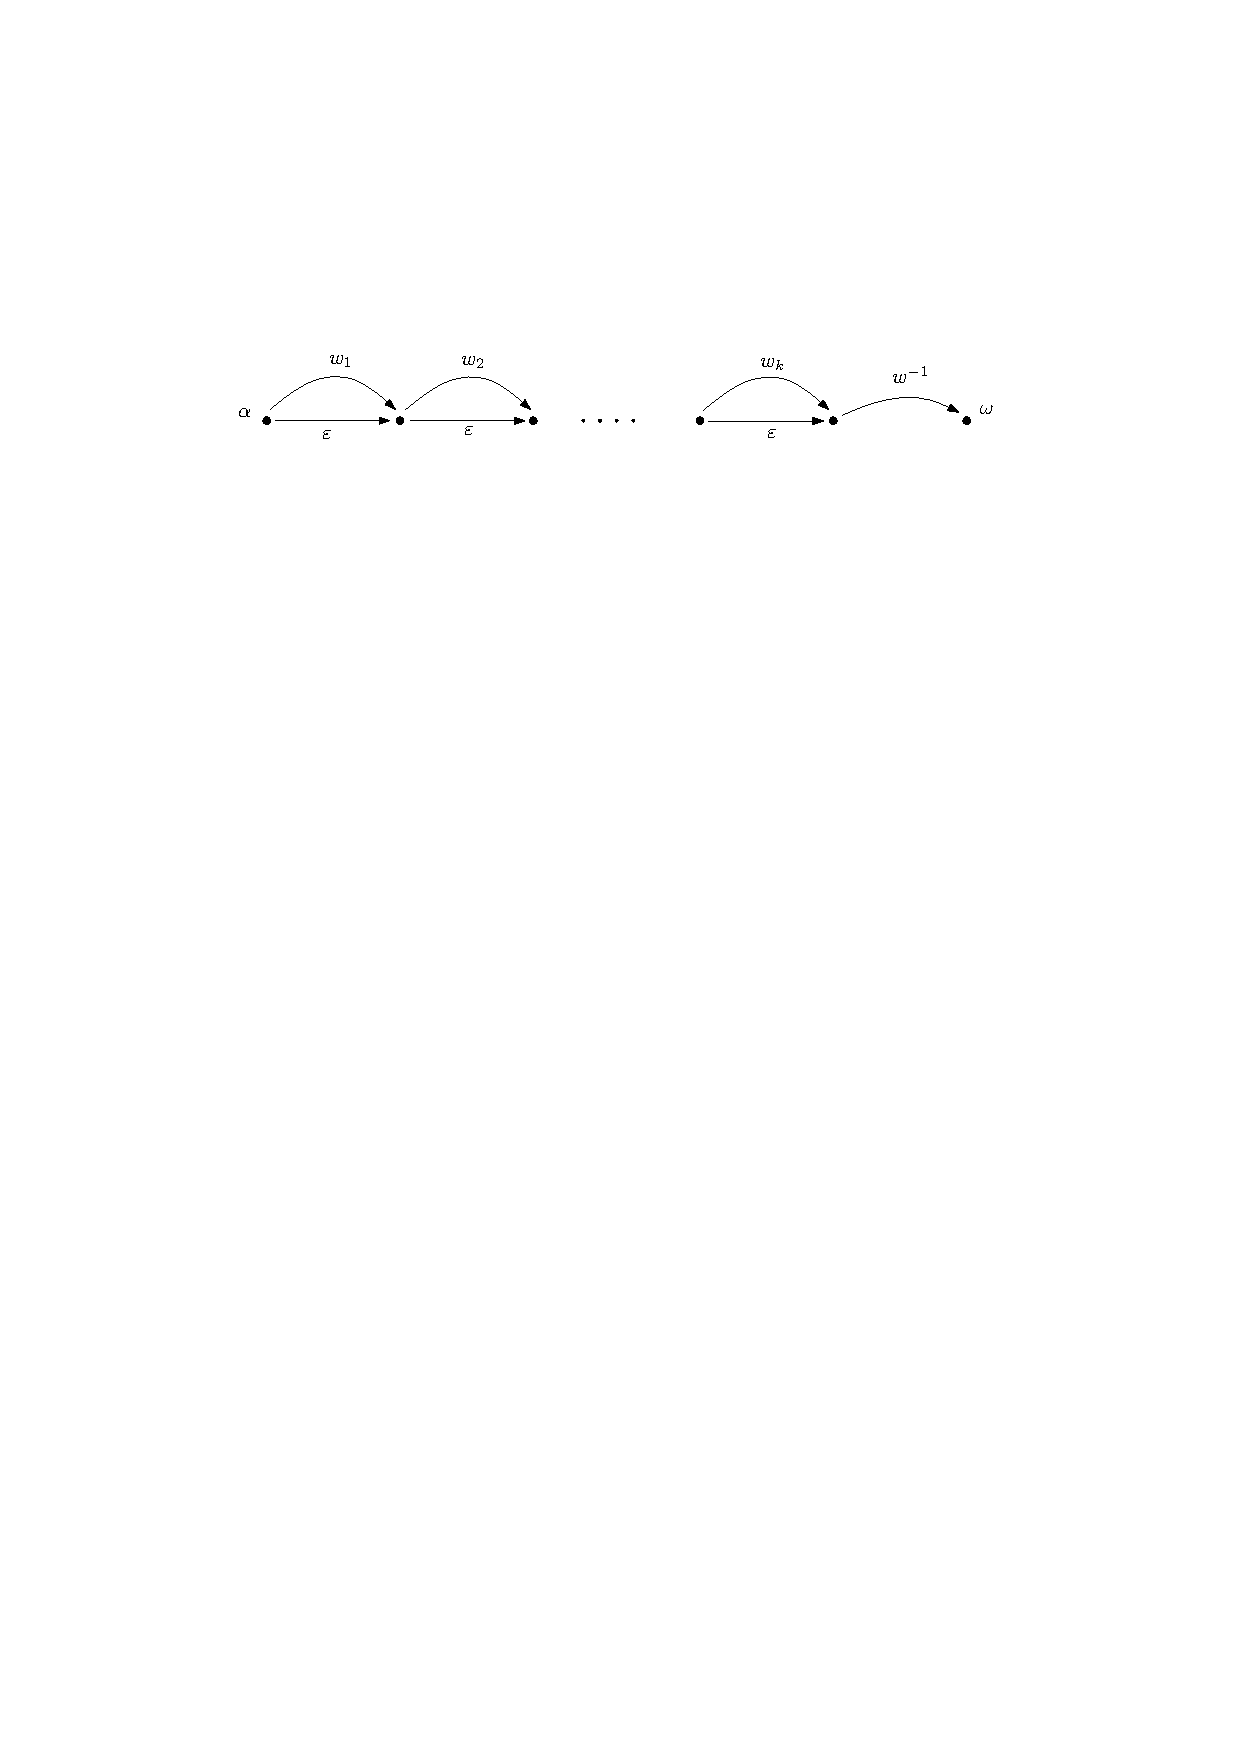
\includegraphics[width=4.5in]{ssp}
 \caption{Graph $\Gamma(w_1,w_2,\ldots,w_k,w)$, Proposition~\ref{pr:reduction_to_agp}.}\label{fi:SSP}
\end{figure}
Since that $\BKP(G)$ $\P$-time reduces to $\SSP(G)$ (see~\cite{Miasnikov-Nikolaev-Ushakov:2014a}), it is only left to prove that $\BSMP(G)$ reduces to $\AGP(G)$. Indeed, let $(w_1,w_2,\ldots,w_k,w,1^n)$ be an input of $\BSMP(G)$. Consider the graph $\Delta=\Delta(w_1,w_2,\ldots,w_k,w,1^n)$ shown in the Fig.~\ref{fi:BSMP}.
\begin{figure}[h]
 \centering
 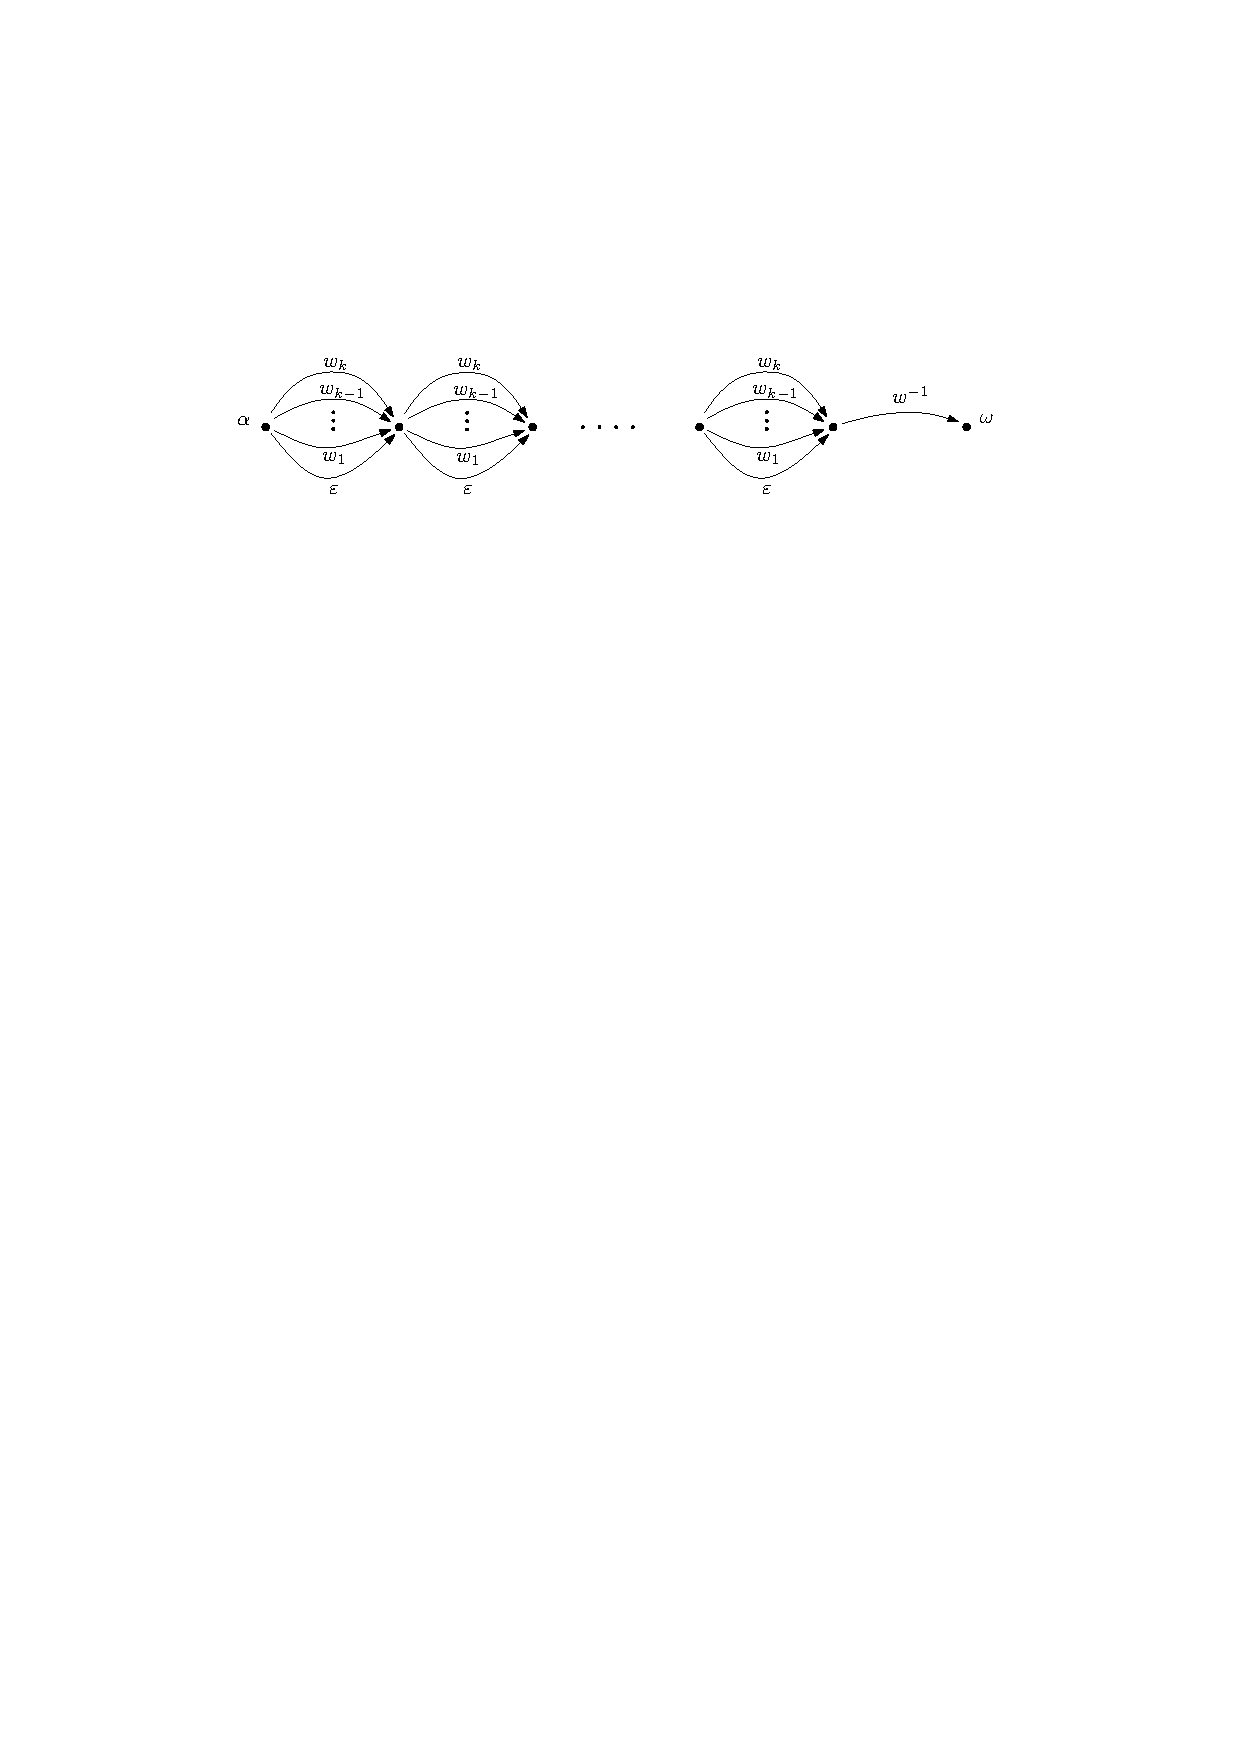
\includegraphics[width=4.5in]{bsmp}
 \caption{Graph $\Delta(w_1,w_2,\ldots,w_k,w,1^n)$, Proposition~\ref{pr:reduction_to_agp}. There are $n+2$ vertices in the graph.}\label{fi:BSMP}
\end{figure}
It is easy to see that $(w_1,w_2,\ldots,w_k,w,1^n)$ is a positive instance of $\BSMP(G)$ if and only if $\Delta$ is a positive instance of $\AGP$.
\end{proof}

Given Proposition~\ref{pr:reduction_to_agp} and results of~\cite{Miasnikov-Nikolaev-Ushakov:2014a}, we immediately see that $\AGP$ is $\NP$-complete in the following cases; certain metabelian groups (finitely generated free metabelian group, wreath products of two infinite abelian groups, Gilbert Baumslag's group $B=\langle a,s,t\mid [a,a^t]=1, [s,t]=1, a^s=aa^t\rangle$, Baumslag--Solitar groups $BS(m,n)$ with $|m|\neq |n|$, $m,n\neq 0$), Thompson's group $F$, $F_2\times F_2$, linear groups $GL(n, \mathbb Z)$ with $n\ge 4$, braid groups $B_n$ with $n\ge 6$, graph groups whose graph contains an induced square $C_4$.

While it still remains to be seen whether $\AGP$ reduces to either of the problems in Proposition~\ref{pr:reduction_to_agp}, we make note of the following two observations. Firstly, in every case when it is known that those problems are $\P$-time, so is $\AGP$, as shown in Propositions~\ref{pr:agp_nilp} and~\ref{pr:agp_hyp}.
The second observation is that for a given group $G$, $\AGP(G)$ $\P$-time reduces to either of the problems $\SSP(G\ast F_2)$ or $\SSP(G\times F_2)$, where $F_2$ is a free group on two free generators.

\begin{proposition}\label{pr:agp_to_ssp_star}
Let $G$ be a finitely generated group, $F_2$ be the $2$-generated free group. Then $\AGP(G)$ is $\P$-time reducible to $\SSP(G\ast F_2)$.
\end{proposition}
\begin{proof}
Let $\Gamma$ be a given directed acyclic graph on $n$ vertices with edges labeled by group words in a generating set $X$ of the group $G$. We start by organizing a topological sorting on $\Gamma$, that is enumerating vertices of $\Gamma$ by symbols $V_1$ through $V_n$ so that if there is a path in $\Gamma$ from $V_i$ to $V_j$ then $i\le j$. This can be done in a time linear in $\size(\Gamma)$ by~\cite{Kahn}. We assume $\alpha=V_1$ and $\omega=V_n$, otherwise discarding unnecessary vertices. We perform a similar ordering of edges, i.e. we enumerate them by symbols $E_1,\ldots, E_m$ so that if there is a path in $\Gamma$ whose first edge is $E_i$ and the last edge $E_j$, then $i\le j$ (considering the dual to $\Gamma$ graph we see that this can be done in time quadratic in $\size(\Gamma)$). For each edge $E_i$, $1\le i\le m$, denote its label by $u_i$, its origin by $V_{o(i)}$, and its terminus by $V_{t(i)}$. We similarly assume that $o(1)=1$ and $t(m)=n$.

Next, we produce in polynomial time $n$ freely independent elements $v_1,\ldots, v_j$ of the free group $F_2$, of which we think as labels of the corresponding vertices $V_1,\ldots, V_n$. For example, $v_j=x^jyx^j$, $j=1,\ldots,n$, suffice.
We claim that
$$g_1 = v_{o(1)}u_1v_{t(1)}^{-1},\ g_2=v_{o(2)}u_2v_{t(2)}^{-1},\ \ldots,\ g_m=v_{o(m)}u_mv_{t(m)}^{-1};\ g=v_{1}v_{n}^{-1}
$$
is a positive instance of $\SSP(G\ast F_2)$ if and only if $\Gamma$ is positive instance of $\AGP(G)$. (See Figure~\ref{fi:agp_to_ssp} for an example.)
\begin{figure}[h]
 \centering
 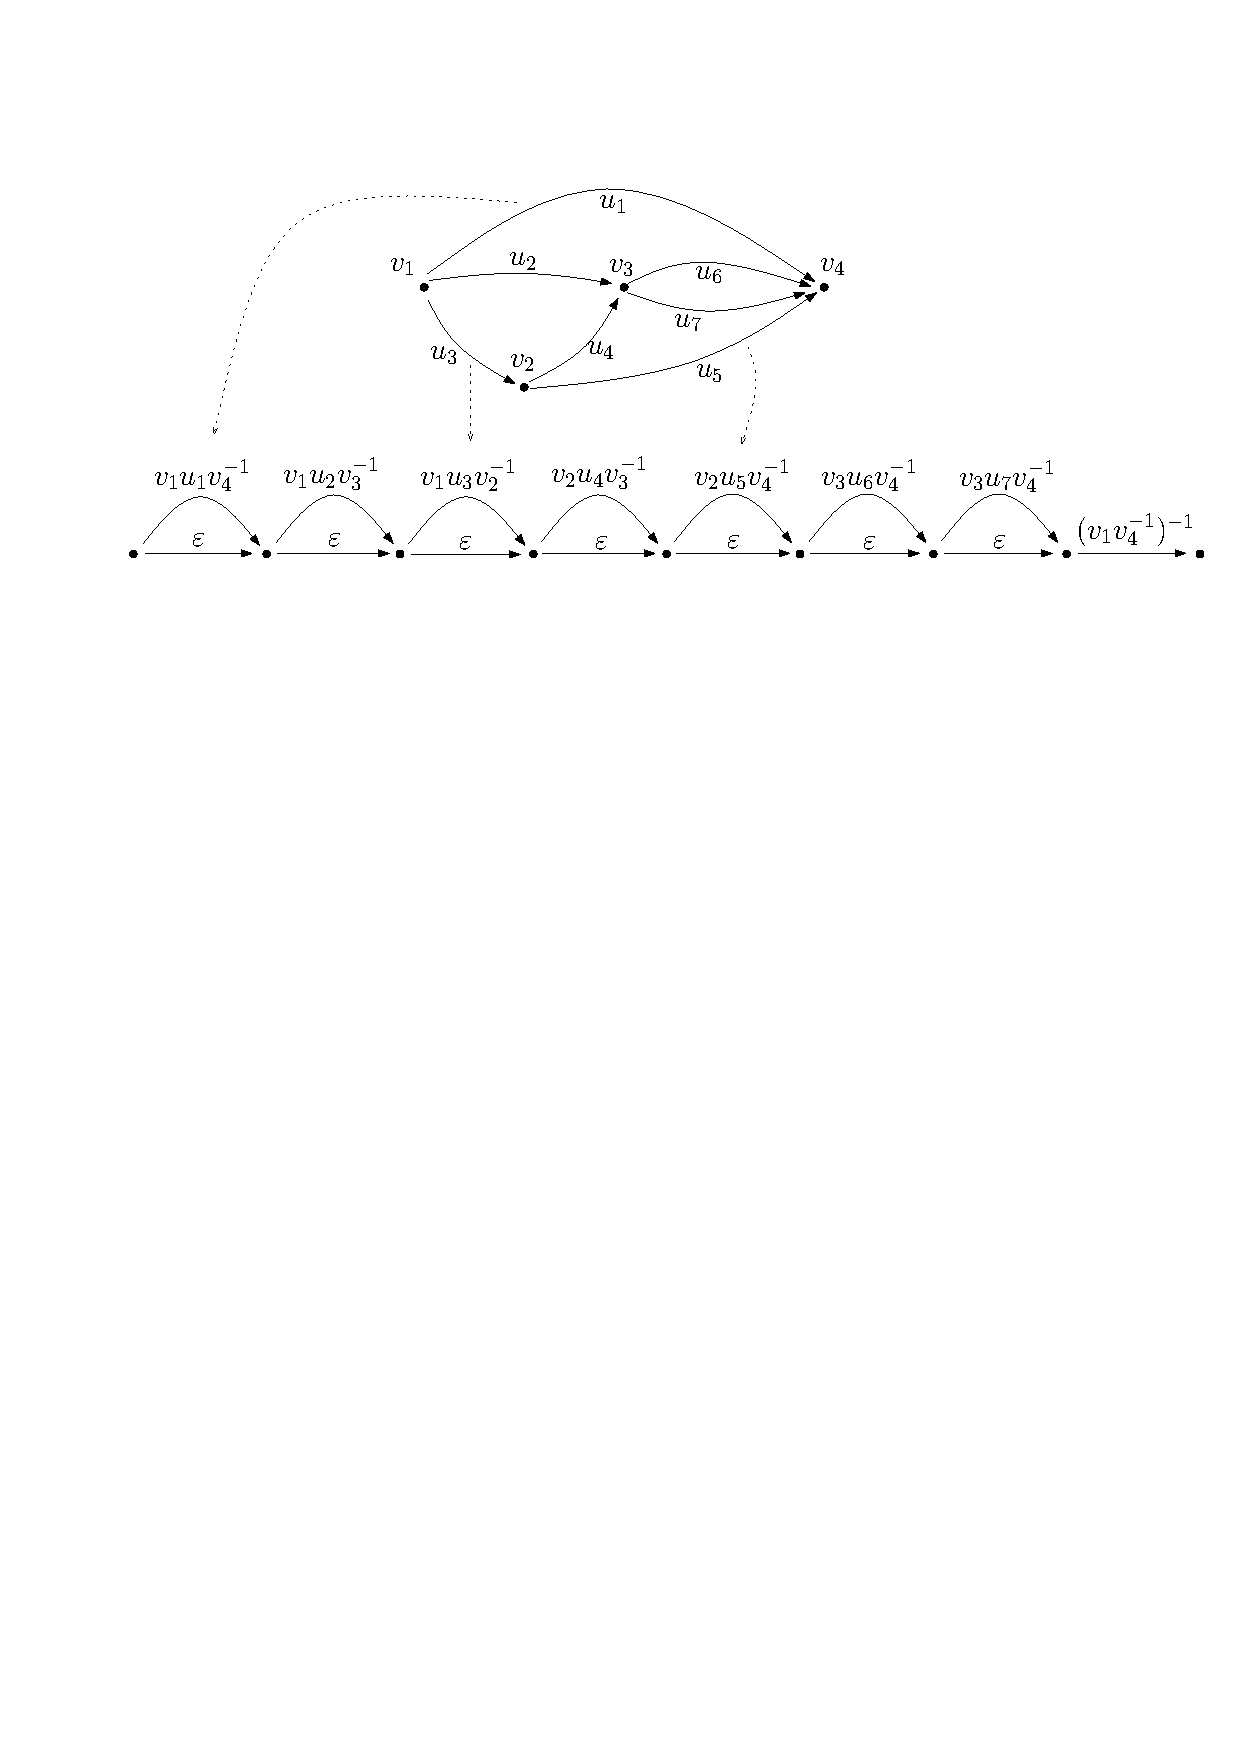
\includegraphics[width=4.5in]{agp_to_ssp}
 \caption{Reduction of $\AGP(G)$ to $\SSP(G\ast F_2)$ and $\SSP(G\times F_2)$. Dotted arrows illustrate the correspondence between edges labeled by $u_i$ and elements $g_i=v_{o(i)}u_iv_{t(i)}^{-1}$.}\label{fi:agp_to_ssp}
\end{figure}
Indeed, suppose there is an edge path $E_{i_1}, \ldots E_{i_k}$ from $\alpha=V_1$ to $\omega=V_n$ in $\Gamma$ with $u_{i_1}\cdots u_{i_k}=1$ in $G$. Note that since the above sequence of edges is a path, for each $1\le \mu\le k-1$, we have $V_{t(\mu)}=V_{o(\mu+1)}$, so $v_{t(\mu)}=v_{o(\mu+1)}$. Then the same choice of elements $g_{i_1},\ldots, g_{i_k}$ gives
\begin{eqnarray*}
g_{i_1}\cdots g_{i_k}&=&(v_{o(i_1)}u_{i_1}v_{t(i_1)}^{-1})
(v_{o(i_2)}u_{i_2}v_{t(i_2)}^{-1})\cdots (v_{o(i_k)}u_{i_k}v_{t(i_k)}^{-1})=\\
&&v_{o(i_1)}u_{i_1}(v_{t(i_1)}^{-1}
v_{o(i_2)})u_{i_2}(v_{t(i_2)}^{-1}v_{o(i_3)})\cdots v_{o(i_k)}u_{i_k}v_{t(i_k)}^{-1}=\\
&&v_{o(i_1)}u_{i_1}u_{i_2}\cdots u_{i_m}v_{t(i_k)}^{-1}=\\
&&v_{o(i_1)}v_{t(i_k)}^{-1}=v_{1}v_{n}^{-1}=g.
\end{eqnarray*}
In the opposite direction, suppose in $G\ast F_2$ the equality
\begin{equation}\label{eq:ssp}
g_{i_1}\cdots g_{i_k}=g,\quad i_1<\ldots<i_k,
\end{equation}
takes place. Consider the $F_2$-component of this equality:
$$
v_{o(i_1)}v_{t(i_1)}^{-1}\cdot v_{o(i_2)}v_{t(i_2)}^{-1}\cdots v_{o(i_k)}v_{t(i_k)}^{-1}=v_1v_n^{-1}.
$$
Since $v_1,\ldots, v_n$ are freely independent, it is easy to see by induction on $k$ that the latter equality only possible if
$$
v_{o(i_1)}=v_1,\ v_{t(i_1)}=v_{o(i_2)},\ v_{t(i_2)}=v_{t(i_3},\ \ldots,\ v_{o(i_{k-1})}=v_{o(i_k)},\ v_{t(i_k)}=v_n,
$$
i.e. edges $E_{i_1}, E_{i_2},\ldots, E_{i_k}$ for a path from $V_1$ to $V_n$ in $\Gamma$. Further, inspecting the $G$-component of the equality~\eqref{eq:ssp}, we get that $u_{i_1}u_{i_2}\cdots u_{i_k}=1$, as required in $\AGP(G)$.
\end{proof}

\begin{proposition}\label{pr:agp_to_ssp_cross}
Let $G$ be a finitely generated group, $F_2$ be the $2$-generated free group. Then $\AGP(G)$ is $\P$-time reducible to $\SSP(G\times F_2)$.
\end{proposition}
\begin{proof}
The proof repeats that of Proposition~\ref{pr:agp_to_ssp_star} with $G\times F_2$ instead of $G\ast F_2$.
\end{proof}

\section{$\AGP$ and $\SSP$ in direct products.}\label{sec:direct_prod}
We show in this section that the direct product of groups may change the complexity of $\AGP$ dramatically, in contrast with results of Section~\ref{sec:free_prod}.
\begin{proposition}\label{pr:agp_cross}
There exist groups $G,H$ such that $\AGP(G),\AGP(H)\in\P$, but $\AGP(G\times H)$ is $\NP$-complete.
\end{proposition}
\begin{proof}
It was shown in~\cite[Theorem 7.4]{Miasnikov-Nikolaev-Ushakov:2014a} that $\BSMP(F_2\times F_2)$ is $\NP$-complete. By Proposition~\ref{pr:reduction_to_agp} it follows that $\AGP(F_2\times F_2)$ is $\NP$-complete, while by Proposition~\ref{pr:agp_hyp} $\AGP(F_2)\in\P$.
\end{proof}

As will be made clear below, Proposition~\ref{pr:agp_to_ssp_cross} is enough to make a similar statement about $\SSP$. However, in the next proposition we organize reduction of $\BSMP(G)$ to $\SSP(G\times \mathbb Z)$, thus simplifying the ``augmenting'' group, which allows to make a slightly stronger statement about complexity of $\SSP$ in direct products.

\begin{proposition}\label{pr:bsmp_to_ssp}
Let $G$ be a finitely generated group. Then $\BSMP(G)$ $\P$-time Cook reduces to $\SSP(G\times \mathbb Z)$.
\end{proposition}
\begin{proof} Let $w_1,w_2,\ldots, w_k, w, 1^n$ be the input of $\BSMP(G)$. We construct graphs $\Gamma_m$, $m=1,\ldots, n$, with edges labeled by elements of $G\times \mathbb Z$ as shown in the Figure~\ref{fi:bsmp_to_ssp}. Note that a path from $\alpha$ to $\omega$ is labeled by a word trivial in $G\times\mathbb Z$ if and only if it passes through exactly $m$ edges labeled by $(w_{i_1},1),\ldots,(w_{i_m},1)$ and $w_{i_1}\cdots w_{i_m}=w$ in $G$. Therefore, the tuple $w_1,\ldots,w_k,1^n$ is a positive instance of $\BSMP(G)$ if and only if at least one of graphs $\Gamma_1,\ldots, \Gamma_n$ is a positive instance of $\SSP(F\times\mathbb Z)$.
\begin{figure}[h]
 \centering
 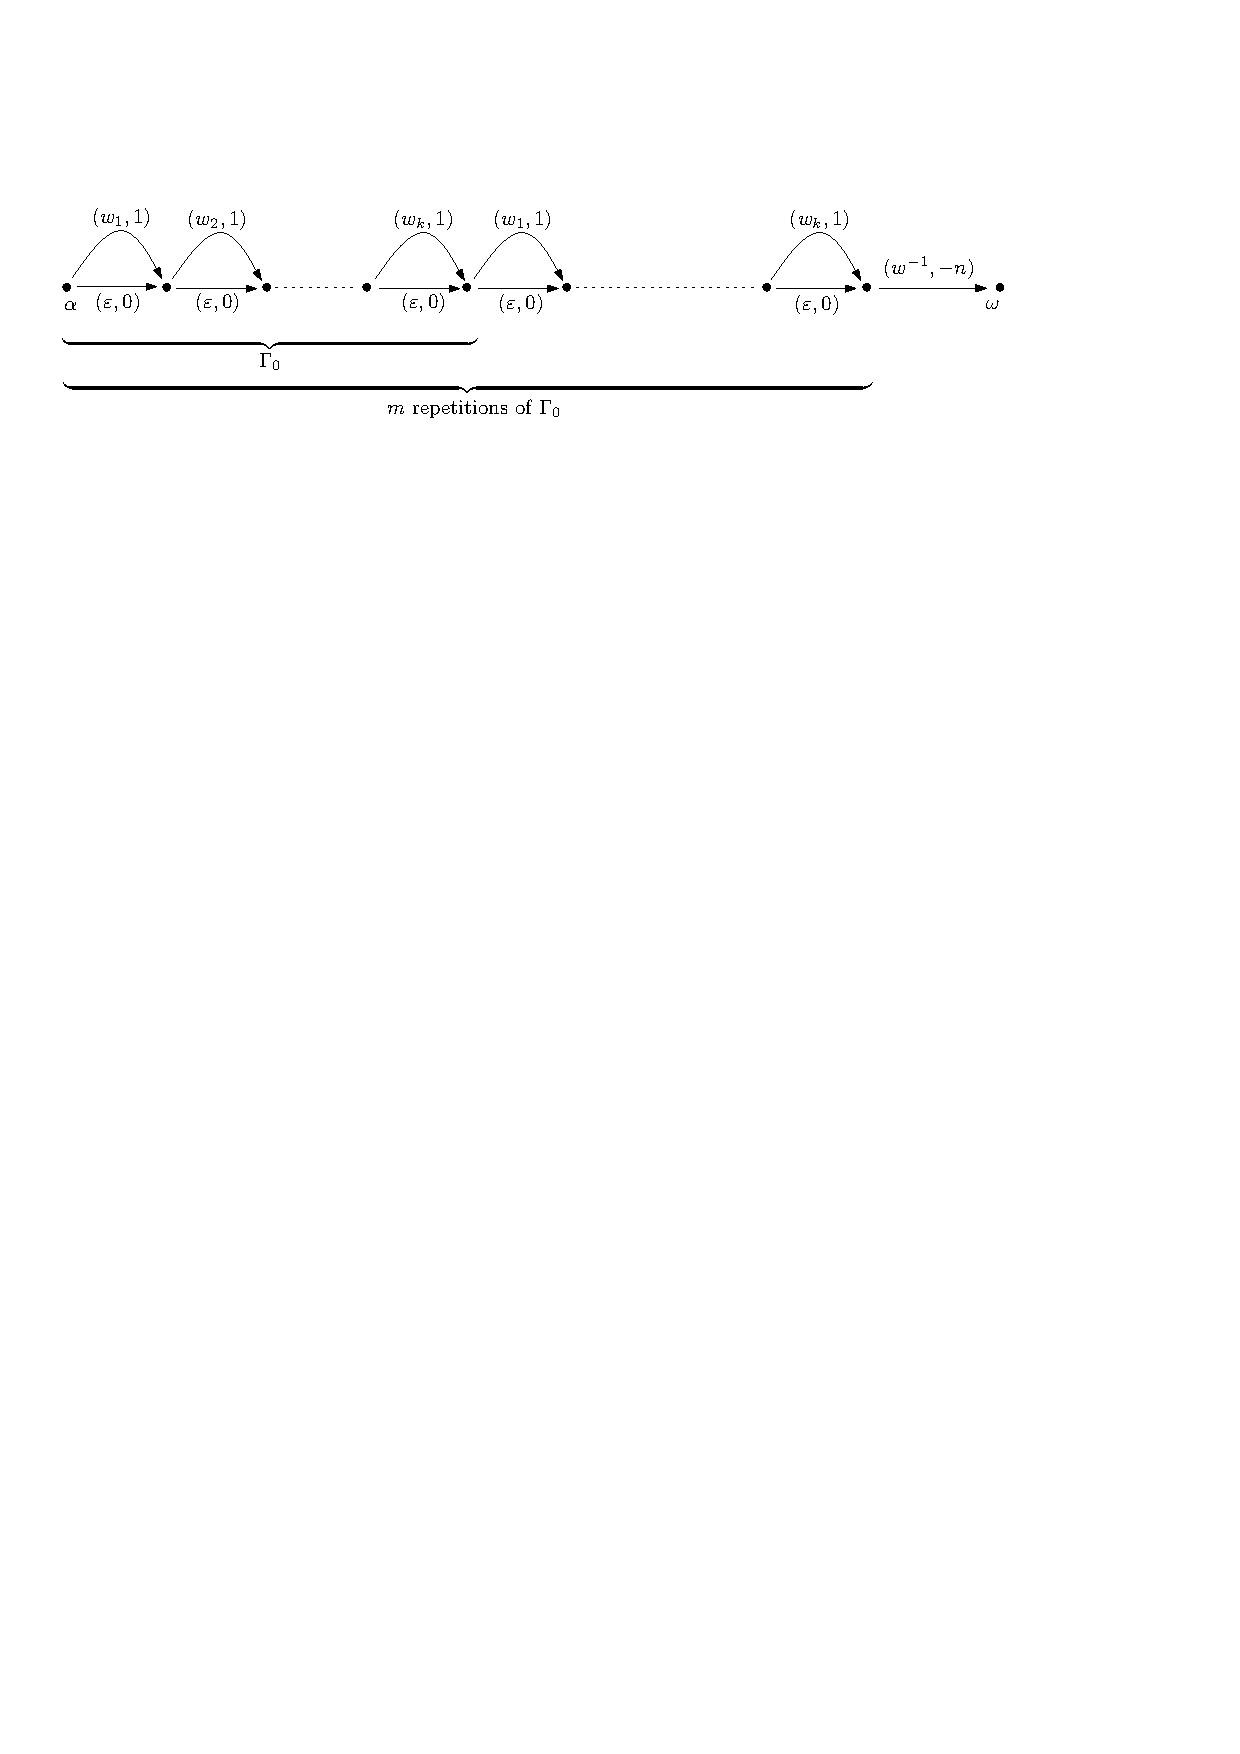
\includegraphics[width=6in]{bsmp_to_ssp}
 \caption{Reduction of $\BSMP(G)$ to $\SSP(G\times \mathbb Z)$. Graph $\Gamma_m$.} \label{fi:bsmp_to_ssp}
\end{figure}
\end{proof}

We put $G=F_2\times F_2$ in the above Proposition~\ref{pr:bsmp_to_ssp} to obtain the following result.
\begin{proposition}\label{pr:ssp_cross}
Let $F_2$ be the $2$-generated free group. $\SSP(F_2\times F_2\times \mathbb Z)$ is $\NP$-complete.
\end{proposition}
\begin{proof}
As we mentioned in the proof of Proposition~\ref{pr:agp_cross}, $\AGP(F_2\times F_2)$ is $\NP$-complete. By Proposition~\ref{pr:bsmp_to_ssp}, the latter $\P$-time Cook reduces to $\SSP((F_2\times F_2)\times\mathbb Z)$). Therefore, the $\SSP(F_2\times F_2\times \mathbb Z)$ is $\NP$-complete.
\end{proof}

The latter proposition answers the question whether a direct product preserves polynomial time $\SSP$.

\begin{corollary}\label{cor:NP_complete_ssp_cross}
There exist finitely generated groups $G,H$ such that $\SSP(G)\in\P$, $\SSP(H)\in\P$ but $\SSP(G\times H)$ is $\NP$-complete.
\end{corollary}
\begin{proof}
By Corollary~\ref{co:F2xZ}, $\AGP(F_2\times\mathbb Z)$ is $\P$-time. Therefore, $\SSP(F_2)$ and $\SSP(F_2\times\mathbb Z)$ are $\P$-time, while
$\SSP(F_2\times (F_2\times \mathbb Z))$ is $\NP$-complete by the above result.
\end{proof}
In the light the above corollary, a natural question to ask is whether $\SSP(F_2\times \mathbb F_2)$ is $\NP$-complete.


\begin{corollary}
$\SSP$ is $\NP$-complete in braid groups $B_n$, $n\ge 8$, special linear groups $SL(n,\mathbb Z)$, $n\ge 5$, graph groups whose graph contains the square pyramid~$\boxtimes$ (also called the wheel graph~$W_5$) as an induced subgraph.
\end{corollary}
\begin{proof}
This follows from Propositions~\ref{pr:bsmp_to_ssp} and~\ref{pr:subgroup} since all of the listed groups contain $F_2\times F_2\times \mathbb Z$ as a subgroup.
\end{proof}


\section{$\AGP$ in free products}\label{sec:free_prod}
\begin{theorem}\label{th:agp_to_factors}
Let $G,H$ be finitely generated groups. Then $\AGP(G*H)$ is $\P$-time Cook reducible to $\AGP(G),\AGP(H)$.
\end{theorem}
\begin{proof}
Let $G$ be given by a generating set $X$, and $H$ by $Y$. Let $\Gamma=\Gamma_0$ be the given acyclic graph labeled by $\Sigma=X\cup X^{-1}\cup Y\cup Y^{-1}\cup\{\varepsilon\}$. Given the graph $\Gamma_k$, $k\in\mathbb Z$, construct graph $\Gamma_{k+1}$ by adding edges to $\Gamma_k$ as follows.

Consider $\Gamma_{k}'$, the maximal subgraph of $\Gamma_k$ labeled by  $X\cup X^{-1}\cup \{\varepsilon\}$ (i.e. the graph obtained by removing all edges labeled by $Y\cup Y^{-1}$).
For each pair of vertices $v_1,v_2\in V(\Gamma_k)$ from the same connected component of $\Gamma_k$, decide whether a word equal to $1$ in $G$ is readable as a label of an oriented path in $\Gamma_k'$, using the solution to $\AGP(G,X)$.
Let $E$ be the set of pairs $(v_1,v_2)\in V(\Gamma_k)\times V(\Gamma_k)$ such that the answer to the above question is positive, and there is no edge $v_1\overset{\varepsilon}{\to}v_2$ in $\Gamma_k.$ Construct the graph $\overline{\Gamma}_k$ by adding edges  $v_1\overset{\varepsilon}{\to}v_2$, $(v_1,v_2)\in E$ to the graph $\Gamma_k$.
Now consider the maximal subgraph $\Gamma_k''$ of $\overline{\Gamma}_k$ labeled by $Y\cup Y^{-1}\cup \{\varepsilon\}$ and perform similar operation using the solution to $\AGP(H,Y)$, obtaining the graph $\overline{\overline{\Gamma}}_k=\Gamma_{k+1}$.
Note that by the construction, $\size(\Gamma_{k+1})<2\size(\Gamma)^2$.

We claim that a word $w$ equal to $1$ in $G*H$ is readable from $\alpha$ to $\omega$ in $\Gamma$ if and only if there is an edge $\alpha\overset{\varepsilon}{\to}\omega$ in the graph $\Gamma_{\size(\Gamma)}$.
Indeed, suppose there is a path in $\Gamma_k$ from $\alpha$ to $\omega$ labeled by a word $w=w_1w_2\cdots w_m$, with $w_j\in \Sigma$ and at least one nontrivial letter among $w_1,\ldots, w_m$, such that $w=1$ in $G*H$.
The normal form theorem for free products guarantees that $w$ has a subword $w'=w_iw_{i+1}\cdots w_j$ of letters in $X\cup X^{-1}\cup \{\varepsilon\}$ or $Y\cup Y^{-1}\cup \{\varepsilon\}$ with $w'=1$ in $G$ or $H$, respectively, with at least one nontrivial letter among $w_i,\ldots,w_j$.
By the construction, the word $w_1\cdots w_{i-1}\varepsilon w_{j+1}\cdots w_m$ is readable as a label of a path in $\Gamma_{k+1}$ from $\alpha$ to $\omega$. Since the graph $\Gamma$ is acyclic, $m< \size(\Gamma)$.
By induction, a word $\varepsilon^{<\size(\Gamma)}$ is readable as a label of an oriented path in $\Gamma_{\size(\Gamma)-1}$ from $\alpha$ to $\omega$.
By the construction, $\Gamma_{\size(\Gamma)}$ contains an edge $\alpha\overset{\varepsilon}{\to}\omega$.
The converse direction of the claim is evident.
%Draw $\varepsilon$-edges in the graph.
\end{proof}

\begin{corollary}\label{cor:ptime_agp}
If $G,H$ are finitely generated groups such that $\AGP(G)$, $\AGP(H)\in\P$ then $\AGP(G*H)\in\P$.
\end{corollary}


\begin{corollary}
$\SSP$, $\BKP$, $\BSMP$, $\AGP$ are polynomial time decidable in free products of finitely generated virtually nilpotent and hyperbolic groups in any finite number.
\end{corollary}

\section{Knapsack problem in free products}\label{sec:knapsack}
It is not clear whether the (unbounded) knapsack problem in general reduces to $\BKP$, or even $\AGP$. However, it was shown in~\cite{Miasnikov-Nikolaev-Ushakov:2014a} that in the case of hyperbolic groups there is indeed such reduction. In light of results of Section~\ref{sec:free_prod}, it is natural to ask whether a similar reduction takes place for free products of groups.

For an element $f$ of a free product of groups $G*H$, let $\|f\|$ denote the {\em syllable length} of $f$, i.e. its geodesic length in generators $G\cup H$ of $G*H$. We say that $f$ is {\em \dumb} if $f$ can be conjugated by an element of $G*H$ into $G\cup H$, i.e.
\begin{equation}\label{eq:simple}
f=u^{-1}f'u,
\end{equation}
where $u\in G*H, \|f'\|\le 1$. Otherwise, we say that $f$ is {\em \nondumb}.

\begin{lemma}\label{le:power}
Let $G,H$ be groups and let an element $f\in G\ast H$ be \nondumb.
%, $f\notin\bigcup_{u\in G*H} G^u\cup H^u$.
Then there are $a_1,\ldots,a_r\in G\cup H$, $b_1,\ldots,b_s\in G\cup H$, $c_1,\ldots,c_t\in G\cup H$, $r+t\le 2\|f\|$, $s\le \|f\|$, such that for every integer $n\ge 3$ the normal form of $f^n$ is
$$
a_1\cdots a_r(b_1\cdots b_s)^{n-2}c_1\cdots c_t.
$$
\end{lemma}
\begin{proof} Follows from the normal form theorem for free products.
\end{proof}

The statement below is, in some sense, a strengthened big-powers condition for a free product.
\begin{proposition}\label{pr:big_power}
There exists a polynomial $p(x)$ with the following property. Let $G,H$ be groups. If for $f_1,f_2,\ldots, f_m, f\in G*H$ there exist non-negative integers $n_1,n_2,\ldots,n_m\in\mathbb Z$ such that
$$
f_1^{n_1}f_2^{n_2}\cdots f_m^{n_m}=f
$$
then there exist such integers $n_1,\ldots,n_m$ with
$$n_i\le p(\|f_1\|+\|f_2\|+\ldots+\|f_m\|+\|f\|)\mbox{ whenever } f_i\mbox{ is \nondumb}.
$$
%for each $i$ such that $f_i$ is \nondumb.
\end{proposition}
\begin{proof}
For each \nondumb\ $f_i$ pass to the form of $f_i^{n_i}$ provided by Lemma~\ref{le:power}. Then inspect the equality in the Cayley graph of $G*H$ with respect to generators $G\cup H$, use pigeonhole principle to find large mutually cancelling pieces of $f_i^{n_i}$ and some $f_j^{n_j}$.
\end{proof}
We assume without loss of generality that $p$ in the above proposition is monotone on $\mathbb{Z}_{\ge 0}$.

\begin{proposition}\label{pr:kp_to_bkp}
If $G,H$ are groups such that $\KP(G),\KP(H)\in\P$, then $\KP(G*H)$ is $\P$-time reducible to $\BKP(G*H)$.
\end{proposition}
\begin{proof}
Let $f_1,f_2,\ldots,f_m,f\in G*H$ be an input of $\KP(G*H)$. For each $f_i$, we can represent $f_i^{n_i}$ by their normal forms using Lemma~\ref{le:power} or simplicity of $f_i$. Suppose some $n_1,n_2,\ldots,n_m$ provide a solution to $\KP$, i.e. $f_1^{n_1}\cdots f_m^{n_m}f^{-1}=1$ in $G*H$. Representing $f^{-1}$ and each $f_i^{n_i}$ by their normal forms and combining like terms we obtain (without loss of generality) a product
\begin{equation}\label{eq:norm_form}
g_1h_1g_2h_2\cdots g_\ell h_\ell=1,
\end{equation}
where each $g_i\in G$ and each $h_i\in H$, and $\ell\le \|f\|+m\cdot (\max\{\|f_i\|\})\cdot p(\max\{\|f_i\|\})$ by Proposition~\ref{pr:big_power}, so $\ell\le N^2p(N)$ where $N$ is the total length of the input (i.e. the sum of word lengths of $f_1,$ \ldots, $f_m,$ $f$). Further, since the product in~\eqref{eq:norm_form} represents the trivial element, it can be reduced to $1$ by a series of eliminations of trivial syllables and combining like terms:
\begin{align*}
g_1h_1g_2h_2\cdots g_\ell h_\ell&=\\
g_1^{(1)}h_1^{(1)}\cdots g_\ell^{(1)}h_\ell^{(1)}&=\\
g_1^{(2)}h_1^{(2)}\cdots g_{\ell-1}^{(2)}h_{\ell-1}^{(2)}&=\\
\ldots=g_1^{(\ell)}h_1^{(\ell)}&=1,\\
\end{align*}
where the product labeled by $(j)$ is obtained from the one labeled by $(j-1)$ by a single elimination of a trivial term and combining the two (cyclically) neighboring terms. Observe that each $g_i^{(j)}$ is (up to a cyclic shift) a product of the form $g_\alpha g_{\alpha+1}\cdots g_\beta$; similarly for $h_i^{(j)}$. Therefore, each $g_i^{(j)}$ is of the form
\begin{equation}\label{eq:g_ij}
g_i^{(j)}=d_{1j}^{\delta_{1j}} d_{2j}^{\delta_{2j}}\cdots d_{k_{ij},j}^{\delta_{k_{ij},j}},
\end{equation}
where each $d_{\mu j}$, $1\le \mu\le k_{ij}$ is either
\begin{itemize}
\item[(NS)] one of the syllables involved in Lemma~\ref{le:power} or ``u'' part of~\eqref{eq:simple}, in which case $\delta_{\mu j}=1$, or
\item[(S)]\label{li:simple} the syllable $f'$ in~\eqref{eq:simple} for some $f_\nu$, in which case $\delta_{\mu j}=n_\nu$.
\end{itemize}
On the one hand, the total amount of syllables $d_{\mu j}$ involved in~\eqref{eq:g_ij} for a fixed $j$ is $k_{1j}+k_{2j}+\cdots +k_{\ell-j+1,j}$. On the other hand, it cannot exceed $k_{11}+k_{21}+\cdots +k_{\ell 1}$
since $g_1^{(j)}$, $g_2^{(j)},$ \ldots, $g_{\ell-j+1}^{(j)}$ are obtained by eliminating and combining elements $g_1$, $g_2$, \ldots, $g_l$. Taking into account that each $k_{i1}\le m+1\le N$, we obtain $k_{1j}+k_{2j}+\cdots +k_{\ell-j+1,j}\le \ell N\le N^3p(N)$.

%total word length of the collection $g_1,\ldots, g_\ell$,


Now, given the equality $g_i^{(j)}=1$ for some $i,j$, if the option~(S) takes place for any $1\le \mu\le k_{ij}$, then the right hand side of the corresponding equality~\eqref{eq:g_ij} can be represented (via a standard conjugation procedure) as a positive instance of the $\KP(G)$ with input of length bounded by $(N k_{ij})^2\le N^8p^2(N)$. Since $\KP(G)\in\P$, it follows that every $n_\nu$ that occurs as some $\delta_{\mu j}$ in some $g_i^{(j)}$ is bounded by a polynomial $p_G(N)$. Similar argument takes place for the $H$-syllables $h_i^{(j)}$, resulting in a polynomial bound $p_H(N)$.

It is only left to note that since for every $1\le \nu\le m$, either $f_\nu$ is non-simple and then $n_\nu$ is bounded by $p(N)$, or it is simple and then $n_\nu$ is bounded by $p_G(N)$ or $p_H(N)$, so every $n_\nu$ is bounded by $p(N)+p_G(N)+p_H(N)$.
%we note that each $g_i$ has the form
% % does this really give algorithmic reduction? Do we have to be able to find p_G,p_H effectively?
\end{proof}

\begin{theorem}\label{th:ptime_kp}
If $G,H$ are groups such that $\AGP(G)$, $\AGP(H)\in\P$ and $\KP(G)$, $\KP(H)\in\P$ then $\KP(G*H)\in\P$.
\end{theorem}
\begin{proof} By Proposition~\ref{pr:kp_to_bkp} $\KP(G*H)$ is $\P$-time reducible to $\BKP(G*H)$. In turn, the latter is $\P$-time reducible to $\AGP(G*H)$ by Proposition~\ref{pr:reduction_to_agp}. Finally, $\AGP(G*H)\in\P$ by Corollary~\ref{cor:ptime_agp}.
\end{proof}
\begin{corollary}
$\KP$ is polynomial time decidable in free products of finitely generated virtually nilpotent and hyperbolic groups in any finite number.
\end{corollary}

%\bibliography{../../main_bibliography}
\bibliography{main_bibliography}
%\printindex

\end{document}

